\subsection{Коммуникация между элементами системы автоматического разворачивания ОбС}

Одной из основных проблем функционирования распределенной обманной системы с множеством ловушек является задача скрытой коммуникации между элементами обманной системы \citep{Peskova2014}. Информацию, собранную о деятельности злоумышленника внутри ловушки-контейнера, нецелесообразно хранить как в самом контейнере, так и на хосте, поддерживающем его функционирование. Возникает угроза компрометации: злоумышленник может обнаружить, удалить и модифицировать данную информацию. Исходя из сказанного следует факт необходимости удаленного сбора. 

Внедрение удаленного сбора информации влечет за собой требования к должной защите данной коммуникации от перехвата. Злоумышленник может проанализировать трафик и обнаружить, что в пересылаемых пакетах содержатся сведения о его собственной деятельности. Можно выделить два способа решения описанной проблемы:
\begin{enumerate}
	\item исключить возможность перехвата пересылаемых данных;
	\item исключить возможность получения информации из пакетов, в случае их перехвата.
\end{enumerate}

Первый способ решения имеет большое количество проблем в реализации. Следует учитывать, что, потенциально, объем передаваемой информации будет достаточно велик. Злоумышленник может производить большое количество действий в контейнере, которые будут порождать массовые изменения в его файловой системе. Все произведенные действия и их результаты необходимо будет передавать на центральный узел. Существующие на данный момент способы скрытой передачи имеют слабую пропускную способность, поскольку базируются либо на стеганографических методах, либо используют встраивание в существующие протоколы (\textit{ICMP}, \textit{IGMP}, \textit{NetBIOS} и т.д.) и не гарантируют полной защиты от перехвата.

Таким образом остается вариант предупреждения возможности получения информации из перехваченных пакетов путем шифрования.

\subsection{Выбор протокола коммуникации}

Учитывая особенности коммуникации между агентом и центральным узлом, наиболее подходящим способом ее реализации является создание своего протокола прикладного уровня, удовлетворяющего специфическим требованиям. Однако реализация своего протокола несет за собой высокую долю вероятности содержания ошибок, поэтому более целесообразным  решением является выбор подходящего протокола прикладного уровня среди существующих.

Требования к соединению между агентом и центральным узлом:
\begin{enumerate}
\item поддержка шифрования;
\item высокая пропускная способность;
\item выбранный протокол взаимодействия должен иметь активную поддержку со стороны команды разработки.
\end{enumerate}

Высокая пропускная способность обусловлена необходимостью к передаче данных малых и средних объемов. Вероятность того, что злоумышленник будет загружать или модифицировать файлы значительного размера крайне мала. В случае, если произойдет изменение файла большого объема, достаточно будет отключить автоматическую отправку с целью исключения затраты ресурсов на передачу и предоставления возможности для отправки других файлов.

Требование к активной поддержке объясняется своевременным реагированием высококвалифицированных специалистов на выявление в протоколе различного рода уязвимостей. Если используемый протокол будет актуален, сравнительно молод и широко распространен, то ему будет уделяться большое количество внимания со стороны информационного сообщества.

Перечисленным требованиям удовлетворяет протокол \textit{WebSocket}. Перечислим преимущества использования данного протокола \citep{Fedorenkov2015WebSocket}:
\begin{itemize}
\item поддерживает криптографические протоколы \textit{SSL/TLS};
\item позволяет организовать полнодуплексную модель связи;
\item имеет низкие требование к сетевым ресурсам и высокую производительность передачи данных. Служебная информация составляет 2 байта на одно сообщение. По результатам сравнения\citep{Fedorenkov2015WebSocket} производительности передачи 1000, 10000 и 100000 пустых сообщений в секунду при помощи протоколов \textit{http} и \textit{WebSocket}, график которого представлен на рис. \ref{fig:websocket_http_compare}, можно сделать вывод, что в сравнении с протоколом \textit{http} протокол \textit{WebSocket} практически в 1000 раз меньше нагружает сеть;
\item протокол является широко используемым. Первая версия протокола вышла в 2008 году, доработан в 2010 и получил распространение в 2011 году. Данный пункт удовлетворяет третьему требованию.
\end{itemize}

\begin{figure}[ht]
\centering
	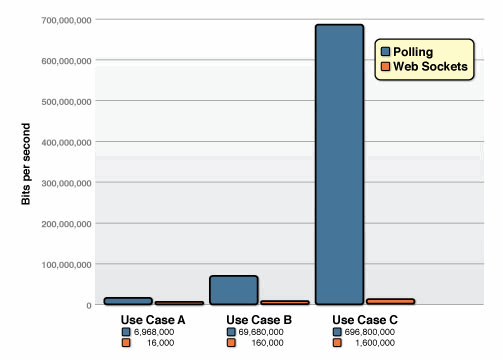
\includegraphics[scale=0.8]{websocket.png}  
	\caption{ Сравнение необходимой пропускной способности сети при передачи пустого сообщения при
помощи обычного \textit{http} соединения и при помощи протокола \textit{WebSocket}}
	\label{fig:websocket_http_compare}
\end{figure}

\subsection{Защита коммуникации}

Выбранный протокол коммуникации поддерживает \textit{SSL} шифрование. В системе будут использоваться два сертификата:
\begin{enumerate}
\item самоподписанный сертификат, закрытый ключ которого будет храниться вне корпоративной сети мероприятия с целью исключения возможности его фальсификации;
\item сертификат центрального узла, который будет использоваться при передаче информации между агентом и центральным узлом. Данный сертификат будет подписан первым сертификатом.
\end{enumerate}

Первый сертификат будет добавлен в агентов в качестве корневого доверенного сертификата.

С целью аутентификации подключаемого к центральному узлу агента   в момент его подключения в начале соединения будет передаваться некоторый секрет. Также данная мера позволяет отслеживать попытки анализа центрального узла со стороны злоумышленника.

Рассмотрим возможные направления развития ситуации:
\begin{itemize}
\item злоумышленник осуществил проникновение в корпоративную сеть и осуществляет перехват пакетов. Учитывая применение шифрования, он не сможет получить их содержимое, однако устанавливает факт необычной передачи данных. При попытке подключения к центральному узлу с целью выявления назначения сервиса и характера пересылаемых пакетов, злоумышленник не сможет пройти процедуру аутентификации, так как не знает необходимого секрета;
\item злоумышленник осуществил проникновение в корпоративную сеть и пытается осуществить \textit{MITM} атаку с целью выявления секрета. Учитывая использование криптографического протокола \textit{SSL}, который обеспечивает аутентификацию, проведение атаки \textit{MITM} невозможно;
\item злоумышленник осуществил проникновение в корпоративную сеть и скомпрометировал хост, содержащий в себе агента, тем самым получив доступ к секрету и исполняемому файлу. Учитывая его информированность о структуре обманной системы ему нецелесообразно выдавать себя за один из ее элементов.
\end{itemize}

Исходя из рассмотренных ситуаций можно сделать вывод о том, что выбранный способ защиты является достаточным в рамках разрабатываемой системы.